\section{The circle problem with the nearest neighbour topology support}
In this task the circle problem is solved using the nearest neighbour topology. This means that the particles no longer represent fully connected topology but each particle rather considers only its specific surrounding.

Figure \ref{fig:2Dcircle_nntopology} shows the results for both 1D and 2D Circle problem with nearest neighbour topology support. In this case the particles only communicate their best global position to three nearest particles.

Figure \ref{fig:2Dcircle_nntopology_inertia} shows the results for both 1D and 2D Circle problem with nearest neighbour topology suppport. It also adds the support for the weighed inertia that influences the value of each particle's velocity. In this case the inertia gradually decreases from value $1.0$ to value $0.4$.

\begin{figure}[!h]
	\centering
		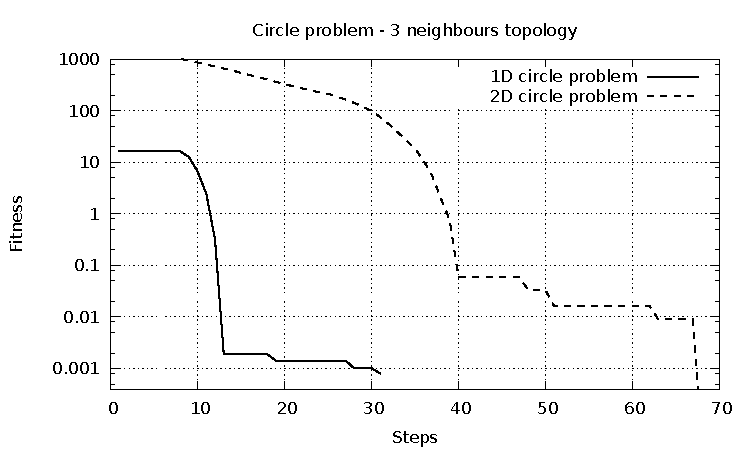
\includegraphics[width=15cm]{img/2a.pdf}
	\caption{2D circle problem with nearest neighbour topology (3 neighbours).}
	\label{fig:2Dcircle_nntopology}
\end{figure}

\begin{figure}[!h]
	\centering
		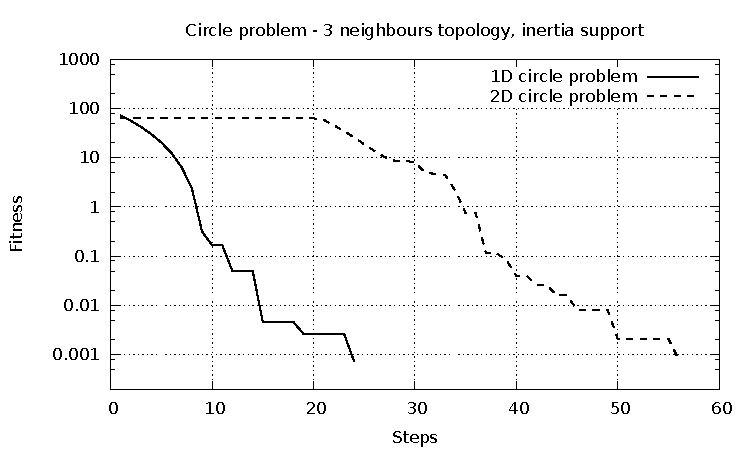
\includegraphics[width=15cm]{img/2b.pdf}
	\caption{2D circle problem with nearest neighbour topology (3 neighbours) and inertia support.}
	\label{fig:2Dcircle_nntopology_inertia}
\end{figure}